% Auto-generated by r_project/simulation/mc_paper.R
% Generated 2026-11-23 12:34 at commit 9e7ae33 (uncommitted changes)
% Monte Carlo rows: commit(s) 7acc201, 2ae035d, f3382b0, bd2f334, 9ceeb42, c1a3c0b, 94dfe82, f1ebed4, 9e7ae33; targets: commit f3382b0,9ceeb42,c1a3c0b,94dfe82,f1ebed4,bd2f334,9e7ae33,817ab68

\begin{figure}[htbp]
\centering
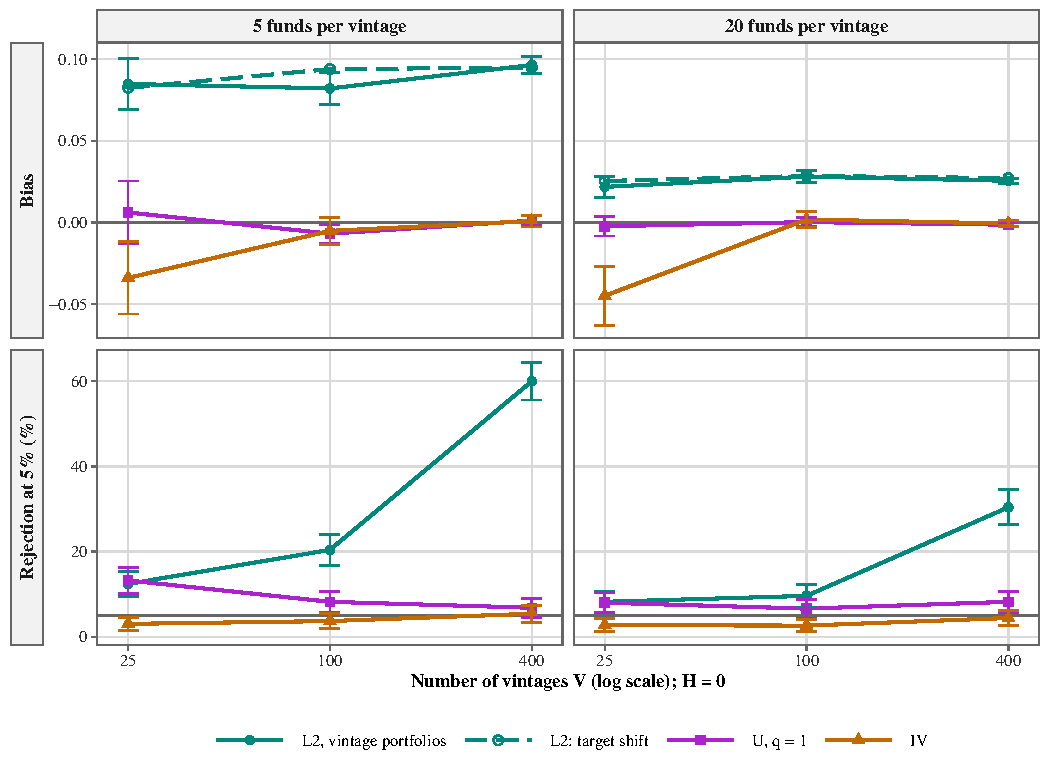
\includegraphics[width=0.85\textwidth]{figure_S3_growing_V.pdf}
\caption{Monte Carlo: more vintages with the same funds per vintage}
\label{fig:mc_growing_v}
\par\vspace{2pt}
{\scriptsize\textit{Notes:} Single-factor $\hat\beta_{MKT}$ (true value 1) at $H=0$ for $V=25$, 100 and 400 consecutive vintages ending 2005 with 5 or 20 funds each, deal model of the cores. Each replication draws its own factor path: whole months of 1967--2021 resampled i.i.d.\ on a calendar from the first vintage to 2021 (100 or 400 vintages do not fit the history). L2 on vintage portfolios with its target shift (the minimizer of the criterion averaged over replications 1--200, minus the true value); $U_{v,H}$ with $q_v=1$; IV as in Table~\ref{tab:mc_size_additions}. The L2 bias does not fall with $V$; it equals the target shift and shrinks with the funds per vintage (the noise tilt, T3/T4), and with a fixed bias and a shrinking SE its rejection rate rises with $V$. Bars: $\pm2$ Monte Carlo SE. 500 replications per design.}
\end{figure}
